From Figure~\ref{fig:SparkStreaming_time_breakdown}, we gained an understanding of how different components of the Spark Streaming architecture contribute to the end-to-end latency. In this section, we focus on optimizing two areas: the overhead of running tasks, and the time it takes for a Receiver to store a block and inform the Driver.

\subsection{Task Overheads}
According to Figure~\ref{fig:SparkStreaming_time_breakdown}, around 11\%, or 7.0ms is spent on average executing a task. However, since our synthetic benchmark performed near-trivial computation, most of the time spent in running the task is due to the overheads in running a task. 

To breakdown the process of running desks, we modified the Receiver so that it generated a block regardless of the number of records received. We then ran the system on empty input, using an application that required a single stage. The application is launched with 1 Receiver, running on the same machine as the Driver. Since there was no input, the computation itself was effectively a no-op. After profiling this workflow, we found that from the Driver's perspective, the average time of running a task, i.e. the time between the task is scheduled and the time between the result is received, was 5.0ms. The difference of 2.0ms was likely due to the fact that there was only 1 Receiver, running on the same machine as the Driver, under a very light load.

As we looked deeper into the 5.0ms, we found that approximately 3.6ms out of this time was in deserializing the task. These numbers suggest that if we can reduce the task deserialization time, there will be a considerable improvement to the overheads of running tasks.

\begin{figure}[t!]
 \begin{center}
   \includegraphics[scale=0.30]{images_graphs/deserialization.eps}
 \end{center}
 \caption{How a task is deserialized on the executor. Examples of new dependencies can be new libraries needed to run the current task.}
 \label{fig:deserialization}
\end{figure}

Having discovered that a significant portion of the time running small tasks is spent in deserialization, we further measured the time it took for individual components of deserialization to complete. Figure \ref{fig:deserialization} summarizes the process of task deserialization on the Executor. The Executor receives a task in the form of an array of bytes called \texttt{serializedTask}. This array is deserialized into a tuple of \texttt{taskFiles}, \texttt{taskJars}, and \texttt{taskBytes}, the first two of which are passed into a method called \texttt{updateDependencies()}, while the latter is further deserialized into a \texttt{task} object. The \texttt{task} object contains information such as the function to run, the RDD to use, and the partition of the RDD to operate on.

\begin{figure}[t!]
 \begin{center}
   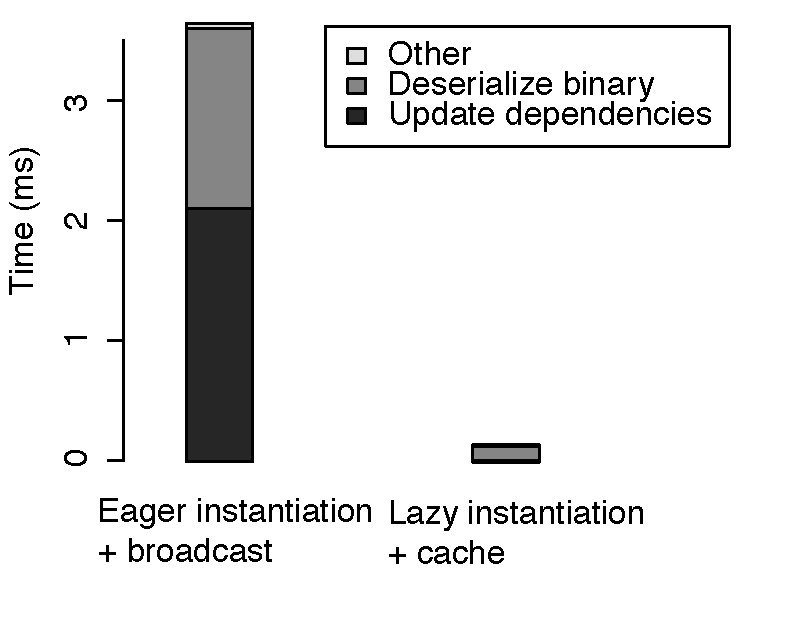
\includegraphics[scale=0.60]{images_graphs/optimizations/graph2/task_deser_micro_illus.pdf}
 \end{center}
 \caption{Breakdown of average time spent deserializing a task before and after adding lazy instantiation of configuration object and caching task binaries.}
 \label{fig:deserialization_times}
\end{figure}

The left part of of Figure \ref{fig:deserialization_times} shows a time breakdown of deserialization. As can be seen in the graph, the majority of the time in this case is in updating dependencies and deserializing \texttt{taskBytes}. We next examine each of these two components in more detail.

\subsubsection{Update Dependencies}
In \texttt{updateDependencies()}, Spark creates a configuration object, and use it when dependencies need to be updated, for example to download additional libraries used by the task. However, this object is created regardless of whether new dependencies are introduced, and this objection creation is very costly in CPU cycles. Since a streaming application rarely introduces new dependencies once it starts to run, this method is incurring unnecessary costs. To solve this problem, we changed the object to be lazily instantiated, so that no cycles are wasted creating the configuration object unless new dependencies are introduced.

\subsubsection{Deserialize Binary}
In order to reduce the amount of duplicate data transferred, Spark wraps the function and the RDD of a task into a broadcast variable, and serializes the broadcast variable as a part of \texttt{taskBinary}. This way, those information are not sent a part of the task, but is pulled by the Executor when it reads the value of the broadcast variable. The advantage of broadcast variable is that once it is pulled by the Executor, the value of the variable is cached in its memory. Therefore, if multiple tasks in the Executor use the same function and RDD, only the first task will need to pull the information from the Driver, and the rest can read it from the cache, reducing network traffic.

This approach, however, is still too wasteful in a streaming environment. Similar to the rarity of new dependencies, the types of RDDs and functions to operate on them change little from batch to batch. With the current approach, one round trip is still required per batch to fetch the function and RDD, even though information could be derived from a previous batch. As the batch interval shrinks, this inefficiency becomes more apparent.

To eliminate this round trip, we experimented with caching of information on the functions and RDDs. The cache is implemented by keeping track of previously broadcasted information on the driver, and resend the previous broadcast variable if possible rather than creating a new one every time. Broadcast variables are automatically cached on the Executor side, so this methodology removes the extraneous communication with the Driver.

\subsection{Block Storage}
As mentioned in Section 2, Spark Streaming heavily uses the producer-consumer pattern, both through its usage of queues with pushing and polling threads as well as the Actor model. This pattern has many advantages, namely modularity, and the ability to explicitly shows bottlenecks in the pipeline. If a downstream processing is slow, a pushback mechanism can be used, where the upstream is blocked from inserting more items into the queue until the queue has free space.

We looked more closely at the section of the system responsible for storing blocks and sending their metadata to the Driver, and found the pushback to be the culprit. More specifically, one thread coalesces records into blocks, and puts them into a queue. Another thread polls the queue, and performs the storage and Driver communication. The consumer in this queue cannot keep up with the producer, introducing delays. To solve this problem, we spawned more threads to act as consumers.

\subsection{Evaluation}
The improvements of the two optimizations in task deserialization are also shown in Figure \ref{fig:deserialization_times}. After the changes, deserialization time for a task decreased from 3.6ms to 0.2ms. The impact of the two changes on overall task runtime is reflected in Figure~\ref{fig:runtime_optimizations}.

\begin{figure}[t!]
 \begin{center}
   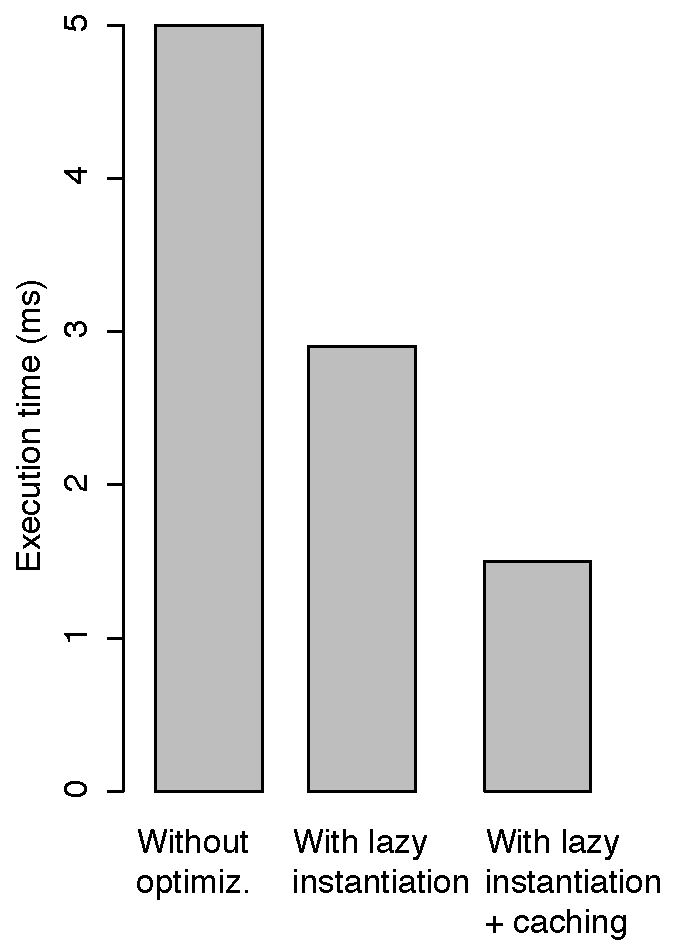
\includegraphics[scale=0.60]{images_graphs/optimizations/graph3/runtime_optimizations.pdf}
 \end{center}
 \caption{Average time spent in running no-op tasks before and after the optimizations in deserialization.}
 \label{fig:runtime_optimizations}
\end{figure}

To show the effect of reducing task runtimes, we performed a micro-benchmark running a single stage with many tasks. The results are shown in Figure \ref{fig:lazy_micro}. For 10K and 100K tasks, lazy instantiation of the configuration object achieves a speedup of 2-3 times.

To examine how the number of consumers storing blocks changes latency, we ran a benchmark with the Receiver and Driver on the same machine, on a data rate of 60MB/s, batch interval of 10ms, and block interval of 2ms. The average time taken to store a block and inform the Driver with respect to the number of consumer threads are shown in Figure {}. As we can see, although two consumers perform better than one consumer, more than two consumers in this case does not necessarily improve the latency.


\subsection{Limitations}
While caching task binaries sound simple in theory, they are more complicated to implement in practice. For example, in our implementation, the Driver caches the serialized format on the function and RDD, and use it to test equality. For serializations across batches to match, we prevented fields such as IDs that are unique across objects to be serialized. While this change does not affect correctness, it will complicate other components such as logging that use those information.

Furthermore, our caching technique only works for batches with single stages. When there are multiple stages, i.e. when shuffles or aggregations are involved, the lineage information of the RDD tends to change from batch to batch, making it difficult to hit a previously broadcasted version.

Finally, the largest limitation to our findings is arguably the fact that we only benchmarked the before and after results on a single machine. This limitation is both due to time constraints as well as volatilities of the distributed environment. For example, since the clocks are synchronoized across machines, the differences between timestamps generated by different machines are less useful, especially when they are in the order of milliseconds.

\begin{figure}[t!]
 \begin{center}
   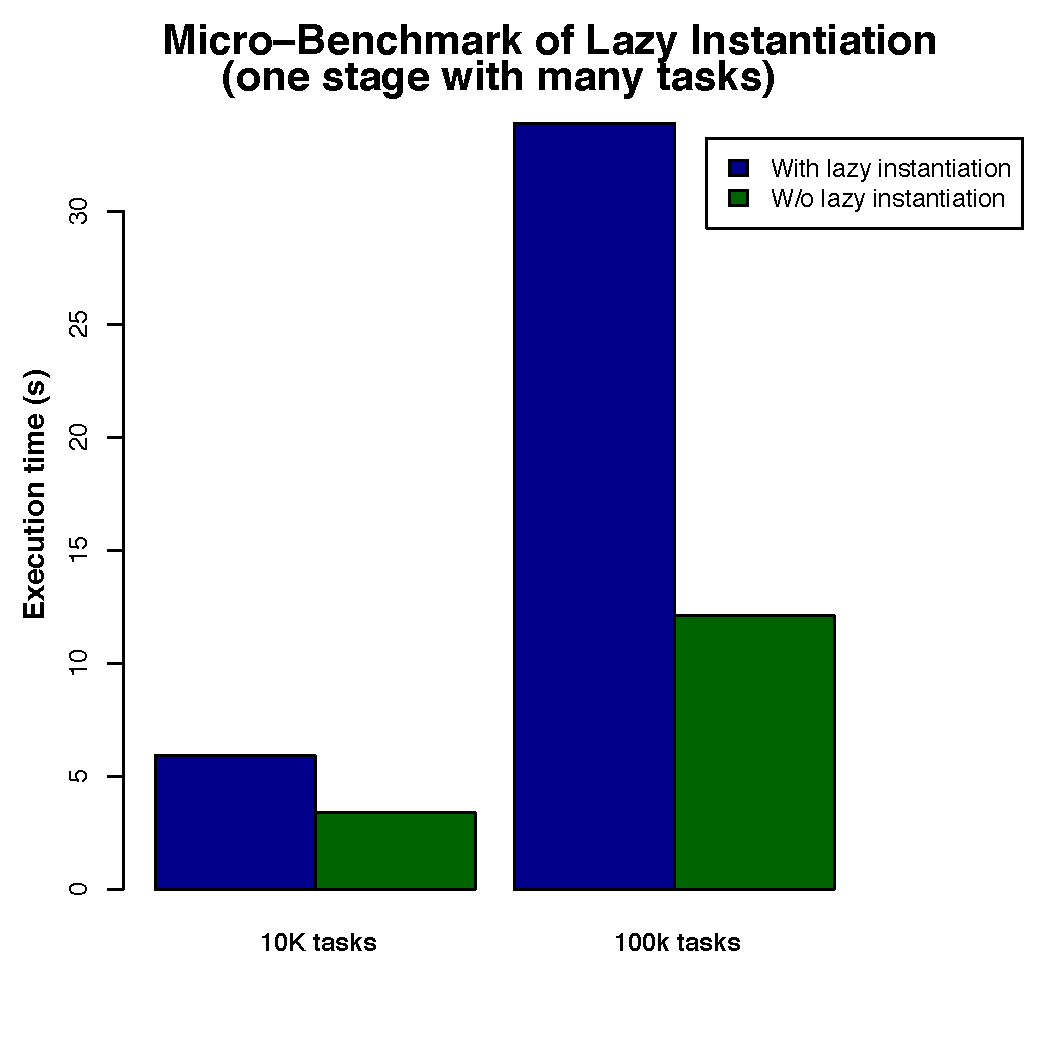
\includegraphics[scale=0.50]{images_graphs/optimizations/graph1/lazy_micro.pdf}
 \end{center}
 \caption{Amount of time spent running a single Spark stage consisting of many tasks without and with lazy instantiation of configuration object.}
 \label{fig:lazy_micro}
\end{figure}
